\documentclass{article}

\usepackage[preprint]{neurips_2024}


\usepackage[utf8]{inputenc} % allow utf-8 input
\usepackage[T1]{fontenc}    % use 8-bit T1 fonts
\usepackage{hyperref}       % hyperlinks
\usepackage{url}            % simple URL typesetting
\usepackage{booktabs}       % professional-quality tables
\usepackage{amsfonts}       % blackboard math symbols
\usepackage{nicefrac}       % compact symbols for 1/2, etc.
\usepackage{microtype}      % microtypography
\usepackage{xcolor}         % colors
\usepackage{amsmath}
\usepackage{multirow}
\usepackage{graphicx}
\usepackage{float}
\usepackage{threeparttable}


\title{When Do Bi-LSTMs Outperform Transformers? A Data-Scale Study for Low-Resource Neural Machine Translation}

\author{%
  Moaz Mahran \\
  University of Waterloo\\
  \texttt{mkgmahra@uwaterloo.ca} \\
  {20964555}
  \And
    Abdullah Shahid \\
  University of Waterloo \\
  \texttt{ashahi38@uwaterloo.ca} \\
  {20985768} \\
  \And
    Sami Yousef\\
  University of Waterloo\\
  \texttt{s22youse@uwaterloo.ca} \\
  {20963803} \\
}


\begin{document}

\maketitle

\begin{abstract}
Transformer-based neural machine translation (NMT) models have achieved state-of-the-art results in high-resource settings, yet their performance and efficiency in genuinely low-resource scenarios remain underexplored. In this paper, we investigate the comparative effectiveness of Bi-LSTM and Transformer architectures across a spectrum of training set sizes ranging from 10k to 200k sentence pairs. Using the IWSLT-2017 German–English dataset, we conduct rigorous hyperparameter tuning with Optuna and evaluate models using BLEU and chrF metrics, as well as compute efficiency in BLEU per GPU-hour and per gradient step. Our results show that Bi-LSTMs outperform Transformers in BLEU at 50k sentence pairs and have better computational efficiency for dataset sizes between 50k–100k, while Transformers regain superiority for bigger datasets. These findings highlight a crossover point in architecture efficacy and underscore the importance of data-aware model selection for low-resource machine translation. We release all code, logs, and trained models to facilitate future research. \footnote{Code, logs, and models are available on Huggingface: \url{https://huggingface.co/samiyousef/bilstm-vs-transormer} and GitHub: \url{https://github.com/samiy803/bistm-vs-transformer}}
\end{abstract}


\section{Introduction}
\label{sec:intro}

Recent breakthroughs in neural machine translation (NMT) have been driven by two major architectures: recurrent models such as Bi-LSTMs \citep{GRAVES2005602} with Luong \citep{luong2015effectiveapproachesattentionbasedneural} attention and attention-only Transformers \citep{vaswani2017attention}. While large-scale studies consistently show that Transformers outperform recurrent models when millions of parallel sentences are available, much less is known about performance when only tens of thousands of sentence pairs exist.

This gap is especially relevant for many truly low-resource languages. For instance, Yoruba, Luganda, and Inuktitut, each spoken by millions but lacking more than a few tens of thousands of parallel sentences. Yoruba in Nigeria has seen limited parallel resources despite over 30–50 million native speakers \citep{adelani2021effect, marote2024bridging}, while Inuktitut faces data sparsity exacerbated by its polysynthetic morphology \citep{roest2020inuktitut, joanis2020nunavut}. In such settings, choosing the wrong architecture can dramatically increase compute cost and training time without yielding gains in translation quality.

In this work, we aim to answer a practical question: \textbf{At what data scale, if any, does a Bi-LSTM model outperform a smaller Transformer model?} Understanding this crossover helps researchers and practitioners working with low-resource corpora decide which architecture offers the best accuracy-to-compute trade-off.

Concretely, we use the IWSLT-2017 German–English corpus \citep{cettolo-etal-2017-overview}, down-sampled to 10k, 50k, 75k, 15k, and 200k, nearing the full 237k sentence pairs, to simulate low-resource settings. We train both Bi-LSTM and Transformer models with the architecture and other hyperparameters optimized by Optuna.

Our contributions are:
\begin{itemize}
  \setlength{\itemsep}{0pt}
  \item A \textbf{learning curve analysis} tracing Bi-LSTM vs. Transformer performance from 10k to 160k training pairs.
  \item A \textbf{cost–efficiency analysis}, measuring BLEU per GPU-hour and gradient updates.
  \item Publicly available reproducible code, logs, and trained models to support future low-resource MT research.
\end{itemize}

We structure the paper as follows. Section~\ref{sec:related-work} surveys prior work on low-resource MT and architectural comparisons. Section~\ref{sec:models} details our Bi-LSTM and Transformer models. Section~\ref{sec:experiments-results} describes our experimental setup and presents the results. Finally, Section~\ref{sec:conclusion} offers conclusions and discusses future research directions.


\section{Related Work}
\label{sec:related-work}

NMT in low-resource settings has received growing attention due to the steep data demands of modern models. Koehn and Knowles highlighted the fragility of NMT with limited data, emphasizing steep learning curves as data decreases \citep{koehn2017challengesneuralmachinetranslation}. Sennrich and Zhang later challenged this pessimism, showing that well-tuned Bi-LSTM models can outperform phrase-based systems with as few as 10k–30k sentence pairs \citep{sennrich2019revisitinglowresourceneuralmachine}. 

 Transformer models dominate high-resource NMT, but are often over-parameterized for small datasets. Several studies have explored scaling effects: research from Google and others has shown that model size, architecture, and optimization interact in complex ways as data increases \citep{hoffmann2022trainingcomputeoptimallargelanguage}. However, most analyses are conducted at the million-sentence scale, leaving gaps in the 10k–200k range that are common for underrepresented languages like Yoruba or Inuktitut. Our work fills this niche by comparing Bi-LSTM and Transformer models side-by-side across low-resource training sizes, with hyperparameter optimization and efficiency analysis.


\section{Models}
\label{sec:models}
We investigate two dominant architectures for neural machine translation: a recurrent neural network with attention (Bi-LSTM) and a Transformer-based encoder-decoder model. Both models are implemented with comparable capacities to ensure a fair comparison under varying data availability constraints. Because both architectures rely on the same sub-word units, we first detail the shared SentencePiece tokenizer used across all experiments.

\subsection{SentencePiece}
\label{subsec:SentencePiece}
SentencePiece is an open-source, language-independent tokenizer that learns a sub-word vocabulary directly from raw UTF-8 text, without requiring any pre-segmentation such as white-space splitting or language-specific rules \citep{kudo2018sentencepiecesimplelanguageindependent}. It frames segmentation as an unsupervised optimization problem and supports both BPE and Unigram Language-Model objectives; in this work we use BPE. Training jointly on the German–English corpus yields a shared vocabulary of 8 000 tokens, into which four reserved IDs are mapped for padding, unknown, start-of-sentence, and end-of-sentence (IDs 0–3 in our implementation). Because SentencePiece emits a self-contained model file, the same tokenizer can be used at training and inference time, ensuring deterministic encoding. Its ability to represent every UTF-8 byte means that even rare characters in true low-resource data can be processed without fallback heuristics, giving consistent coverage across languages and simplifying downstream model design.

\subsection{Transformer}
\label{subsec:transformer}
The Transformer model is a reduced version of the original architecture proposed by Vaswani et al. \citep{vaswani2017attention}. Each layer includes multi-head self-attention, a feed-forward sublayer with residual connections, and layer normalization. The model uses fixed sinusoidal positional encoding, which is added to token embeddings to preserve order information, and it is trained with the Adam optimizer and Noam scheduler, as proposed in the original paper.

Like the Bi-LSTM model, the Transformer shares the same 8,000-token BPE vocabulary for fair comparison. To ensure architectural parity, the Transformer-small was designed to match the Bi-LSTM in training budget. This allows us to isolate the effect of architecture type when comparing model performance in low-resource settings.

Rather than using fixed dimensions, we tune the number of encoder and decoder layers, model dimensionality, attention heads, and related parameters using Optuna. Hyperparameters such as layer depth, model dimension, and learning rate scaling are tuned independently for each training set size. The search space and optimal parameters per dataset size are listed in Table~\ref{table:transformer-hyperparameter-tuning}.

\subsection{Bi-LSTM}
\label{subsec:bi-lstm}
The Bi-LSTM model follows a standard encoder-decoder architecture with attention. The encoder consists of bidirectional LSTM layers that capture both past and future context, producing contextual embeddings for each input token. The decoder is a two-layer unidirectional LSTM that operates autoregressively to generate target tokens one at a time. At each decoding step, Luong-style global attention \citep{luong2015effectiveapproachesattentionbasedneural} is applied, computing a context vector based on alignment between the decoder state and encoder outputs. This context is concatenated with the decoder state to form the attention-aware representation used for prediction.

Outputs are then passed through a linear projection and softmax layer over the shared 8,000-token byte-pair encoded (BPE) vocabulary. All layers apply dropout regularization, and weights are optimized using Adam with gradient clipping and a StepLR scheduler. Rather than using fixed parameters, we tune the number of layers, hidden size, embedding size, dropout, and other parameters using Optuna. Full hyperparameter configurations are provided in Table~\ref{table:bilstm-hyperparameter-tuning}. This architecture has proven effective for low-resource neural machine translation in prior work \citep{sennrich2019revisitinglowresourceneuralmachine}.


\section{Hyperparameter Tuning}
\label{sec:hyperparameter-tuning}

We perform hyperparameter optimization using Optuna \citep{akiba2019optunanextgenerationhyperparameteroptimization}, conducting a separate study for each model type (Bi-LSTM or Transformer) and dataset size. All studies share the same training and validation splits, and apply a fixed SentencePiece tokenizer across all trials for consistency.

To reduce computational cost on smaller datasets, we limit both the number of trials and the number of training epochs per trial in proportion to dataset size. Table~\ref{table:optuna-budgets} summarizes these budgets. Each trial is trained with a fixed batch size (2048 for Bi-LSTM, 1024 for Transformer) and evaluated on BLEU score using beam search decoding. Section ~\ref{subsec:training} provides more details on training and evaluation.


\begin{table}[H]
  \small
  \centering
  \caption{\textbf{Bi-LSTM hyperparameter tuning.} Both models used the same number of trials and epochs per trial.}
  \label{table:optuna-budgets}
  \begin{tabular}{lcccccc}
    \toprule
      & 10k & 50k & 75k & 100k & 150k & 200k \\
      Number of trials & 15 & 20 & 25 & 25 & 25 & 25\\
      Epochs per trial & 4 & 5 & 5 & 8 & 10 & 10 \\
    \bottomrule
  \end{tabular}
\end{table}



Each Optuna study is warm-started by enqueuing the best hyperparameters from the previous (smaller) dataset’s study. This sequential initialization biases the search toward high-performing regions of the hyperparameter space, accelerating convergence and reducing redundant exploration. Trials are evaluated using median-pruning based on BLEU improvements, with pruning configured to activate after 5 startup trials and 2 warm-up steps.

We tune both architectural and optimization hyperparameters. For Bi-LSTMs, this includes embedding and hidden sizes, dropout, and learning rate scheduler parameters. For Transformers, the search space includes model dimensionality, number of heads and layers, warmup steps, and a scaling factor for the learning rate (held constant at 1.0 otherwise). In both cases, we use the Adam optimizer and apply either a StepLR or Noam learning rate schedule depending on model type. The search space and optimal values per dataset size are shown in Tables~\ref{table:bilstm-hyperparameter-tuning} and~\ref{table:transformer-hyperparameter-tuning}.


\begin{table}[H]
  \small
  \centering
  \caption{\textbf{Bi-LSTM hyperparameter tuning.}  
  Search spaces are written as \emph{min–max (step)} or an explicit set.}
  \label{table:bilstm-hyperparameter-tuning}
  \resizebox{\textwidth}{!}{%
  \begin{tabular}{lccccccc}
    \toprule
    \multirow{2}{*}{Parameter}
      & \multirow{2}{*}{Search space}
      & \multicolumn{6}{c}{Best value by training-set size (sentence pairs)} \\
    \cmidrule(lr){3-8}
      & & 10k & 50k & 75k & 100k & 150k & 200k \\
    \midrule
    \texttt{emb\_size}            & 128 -- 512 (64)        & 256 & 320 & 320 & 448 & 384 & 384 \\
    \texttt{hidden\_size}         & 256 -- 1024 (128)      & 1024 & 896 & 1024 & 1024 & 1024 & 1024 \\
    \texttt{num\_layers}          & 1 -- 3                 & 2 & 2 & 2 & 2 & 2 & 2 \\
    \texttt{dropout}              & 0.10 -- 0.30           & 0.300 & 0.288 & 0.264 & 0.253 & 0.239 & 0.239 \\
    \texttt{lr}                   & $3\!\times\!10^{-4}$ -- $5\!\times\!10^{-3}$ (log) & 3.28e-3 & 3.25e-3 & 2.69e-3 & 2.86e-3 & 4.50e-3 & 4.50e-3 \\
    \texttt{weight\_decay}        & $1\!\times\!10^{-6}$ -- $1\!\times\!10^{-4}$ (log) & 3.56e-6 & 1.27e-5 & 5.61e-6 & 4.30e-6 & 4.44e-6 & 4.44e-6 \\
    \texttt{clip\_norm}           & 0.10 -- 1.00           & 0.175 & 0.958 & 0.542 & 0.555 & 0.723 & 0.723 \\
    \texttt{eps}                  & $1\!\times\!10^{-9}$ -- $1\!\times\!10^{-6}$ (log) & 5.36e-8 & 4.59e-8 & 5.25e-8 & 8.71e-9 & 1.42e-8 & 3.66e-8 \\
    $\beta_{1}$                   & 0.80 -- 0.99 (0.01)    & 0.88 & 0.91 & 0.9 & 0.95 & 0.85 & 0.84 \\
    $\beta_{2}$                   & 0.90 -- 0.999 (0.001)  & 0.97 & 0.999 & 0.998 & 0.999 & 0.999 & 0.989 \\
    \texttt{scheduler\_step\_size}& 10 -- 40               & 36 & 14 & 15 & 20 & 9 & 9 \\
    \texttt{scheduler\_gamma}     & 0.70 -- 0.90           & 0.766 & 0.334 & 0.253 & 0.438 & 0.269 & 0.269 \\
    \bottomrule
  \end{tabular}}
\end{table}


\begin{table}[H]
  \small
  \centering
  \caption{\textbf{Transformer hyperparameter tuning.}  
  Base learning-rate is set by \texttt{lr\_scale}.}
  \label{table:transformer-hyperparameter-tuning}
  \resizebox{\textwidth}{!}{%
  \begin{tabular}{lccccccc}
    \toprule
    \multirow{2}{*}{Parameter}
      & \multirow{2}{*}{Search space}
      & \multicolumn{6}{c}{Best value by training-set size (sentence pairs)} \\
    \cmidrule(lr){3-8}
      & & 10k & 50k & 75k & 100k & 150k & 200k \\
    \midrule
    \texttt{d\_model}             & 256 -- 512 (128)       & 256 & 512 & 512 & 256 & 256 & 384 \\
    \texttt{nhead}                & \{4, 8\}            & 4 & 4 & 8 & 4 & 4 & 8 \\
    \texttt{num\_layers}          & 2 -- 4                 & 4 & 3 & 4 & 3 & 3 & 4 \\
    \texttt{dropout}              & 0.10 -- 0.30           & 0.285 & 0.104 & 0.256 & 0.147 & 0.147 & 0.175 \\
    \texttt{lr\_scale}            & 0.20 -- 2.00 (log)     & 0.955 & 0.813 & 1.825 & 1.365 & 1.365 & 1.674 \\
    \texttt{weight\_decay}        & $1\!\times\!10^{-6}$ -- $1\!\times\!10^{-4}$ (log) & 3.62e-5 & 1.14e-5 & 6.02e-5 & 3.73e-5 & 3.73e-5 & 5.64e-5 \\
    \texttt{clip\_norm}           & 0.10–1.00           & 0.619 & 0.807 & 0.635 & 0.443 & 0.443 & 0.842 \\
    \texttt{eps}                  & $1\!\times\!10^{-9}$ -- $1\!\times\!10^{-6}$ (log) & 1.46e-7 & 7.86e-9 & 6.85e-7 & 1.10e-9 & 1.10e-9 & 7.85e-7 \\
    $\beta_{1}$                   & 0.80 -- 0.99 (0.01)    & 0.83 & 0.86 & 0.90 & 0.94 & 0.94 & 0.91 \\
    $\beta_{2}$                   & 0.90 -- 0.999 (0.001)  & 0.927 & 0.948 & 0.947 & 0.930 & 0.930 & 0.934 \\
    \texttt{warmup\_steps}        & 400 -- 800 (50)        & 450 & 600 & 750 & 550 & 550 & 500 \\
    \bottomrule
  \end{tabular}}
\end{table}


\section{Experiments \& Results}
\label{sec:experiments-results}

\subsection{Training \& Evaluation}
\label{subsec:training}

\paragraph{Training Protocol}
All models were trained on a single NVIDIA H100 SXM GPU. For the Bi-LSTM experiments, we used a batch size of 2048 and ran for up to 2 000 gradient‐update steps or one GPU‐hour, whichever came first. The Transformer models could not fit a batch size of 2048 in memory, so we instead used a batch size of 1024 and doubled the maximum number of steps to 4 000, again capped at one GPU‐hour. We optimized both architectures with Adam (Bi-LSTM: initial lr from Optuna; Transformer: Noam schedule with Optuna’s lr\_scale), applied gradient clipping to a norm suggested by Optuna, and used dropout as specified in Section \ref{sec:models}. Checkpoints were saved every 500 steps, and we retained the single checkpoint with the highest validation BLEU for each run.
\paragraph{Evaluation Strategy}
\label{subsec:evaluation}
During inference we applied beam search with beam size 4 and no length penalty. We compute corpus BLEU and chrF using SacreBLEU \citep{post-2018-call} (version 2.5.1) to ensure reproducibility. Rather than using the final checkpoint, we report each model’s best validation BLEU (i.e.\ early‐stopping by maximum validation score) to avoid penalizing runs that slightly overfit late in training.

\paragraph{Efficiency Analysis}  
\label{subsec:efficiency}
We assess model efficiency using two metrics: BLEU per GPU-hour and BLEU per gradient step. As shown in Table~\ref{table:bleu-gpu-hour}, the Bi-LSTM model exhibits markedly higher BLEU/GPU-hour at intermediate dataset sizes (50k-100k), peaking at 244.27 BLEU/GPU-hour on 50k pairs, compared to the Transformer's 14.95. This suggests superior compute efficiency in mid-resource settings. Similarly, Table~\ref{table:bleu-gpu-step} highlights the Bi-LSTM’s step-wise advantage, achieving over 3× higher BLEU/step at 50k-100k, despite a simpler architecture. However, the Transformer closes this gap as data scale increases, achieving the highest absolute BLEU at 200k while maintaining competitive BLEU/step. These results reinforce the importance of data-aware architectural choices when optimizing for efficiency under compute or time constraints.



\subsection{Results}
\label{subsec:results}
Figure~\ref{fig:crossover} presents BLEU and chrF scores for Bi-LSTM and Transformer models across the six training-set sizes. At the smallest scale (10k pairs), the Transformer achieves the highest BLEU (7.89) and chrF, outperforming the Bi-LSTM baseline (2.93 BLEU). However, by 50k pairs, the Bi-LSTM overtakes the Transformer, reaching 18.55 BLEU versus 9.71, with a substantial chrF improvement as well. This marks the crossover point in model effectiveness under limited data.

The Bi-LSTM maintains an advantage through 50k–75k pairs, peaking at 22.09 BLEU at 75k. Beyond this range, the Transformer steadily surpasses the recurrent model, reaching 25.60 BLEU at 75k and ultimately 29.44 BLEU at 200k, consistent with the expected scaling behavior of attention-based architectures on larger corpora. These trends confirm that model choice is highly data-dependent: Bi-LSTMs can outperform Transformers in low-to-mid-resource regimes, while Transformers dominate as the dataset approaches 200k pairs.

These results illustrate a trade-off: Bi-LSTMs provide strong low-resource performance and efficiency, while Transformers excel when sufficient training data is available. Further research is needed to determine whether the sharp performance jump at 50k is a consistent trend or an isolated outlier. Sampling the lower end of the data range more finely, for example from 5k to 75k in 5k increments, would clarify whether there is a true low-resource regime where Bi-LSTMs consistently outperform Transformers or if the observed crossover is a one-off effect.

\begin{figure}[ht]
\centering
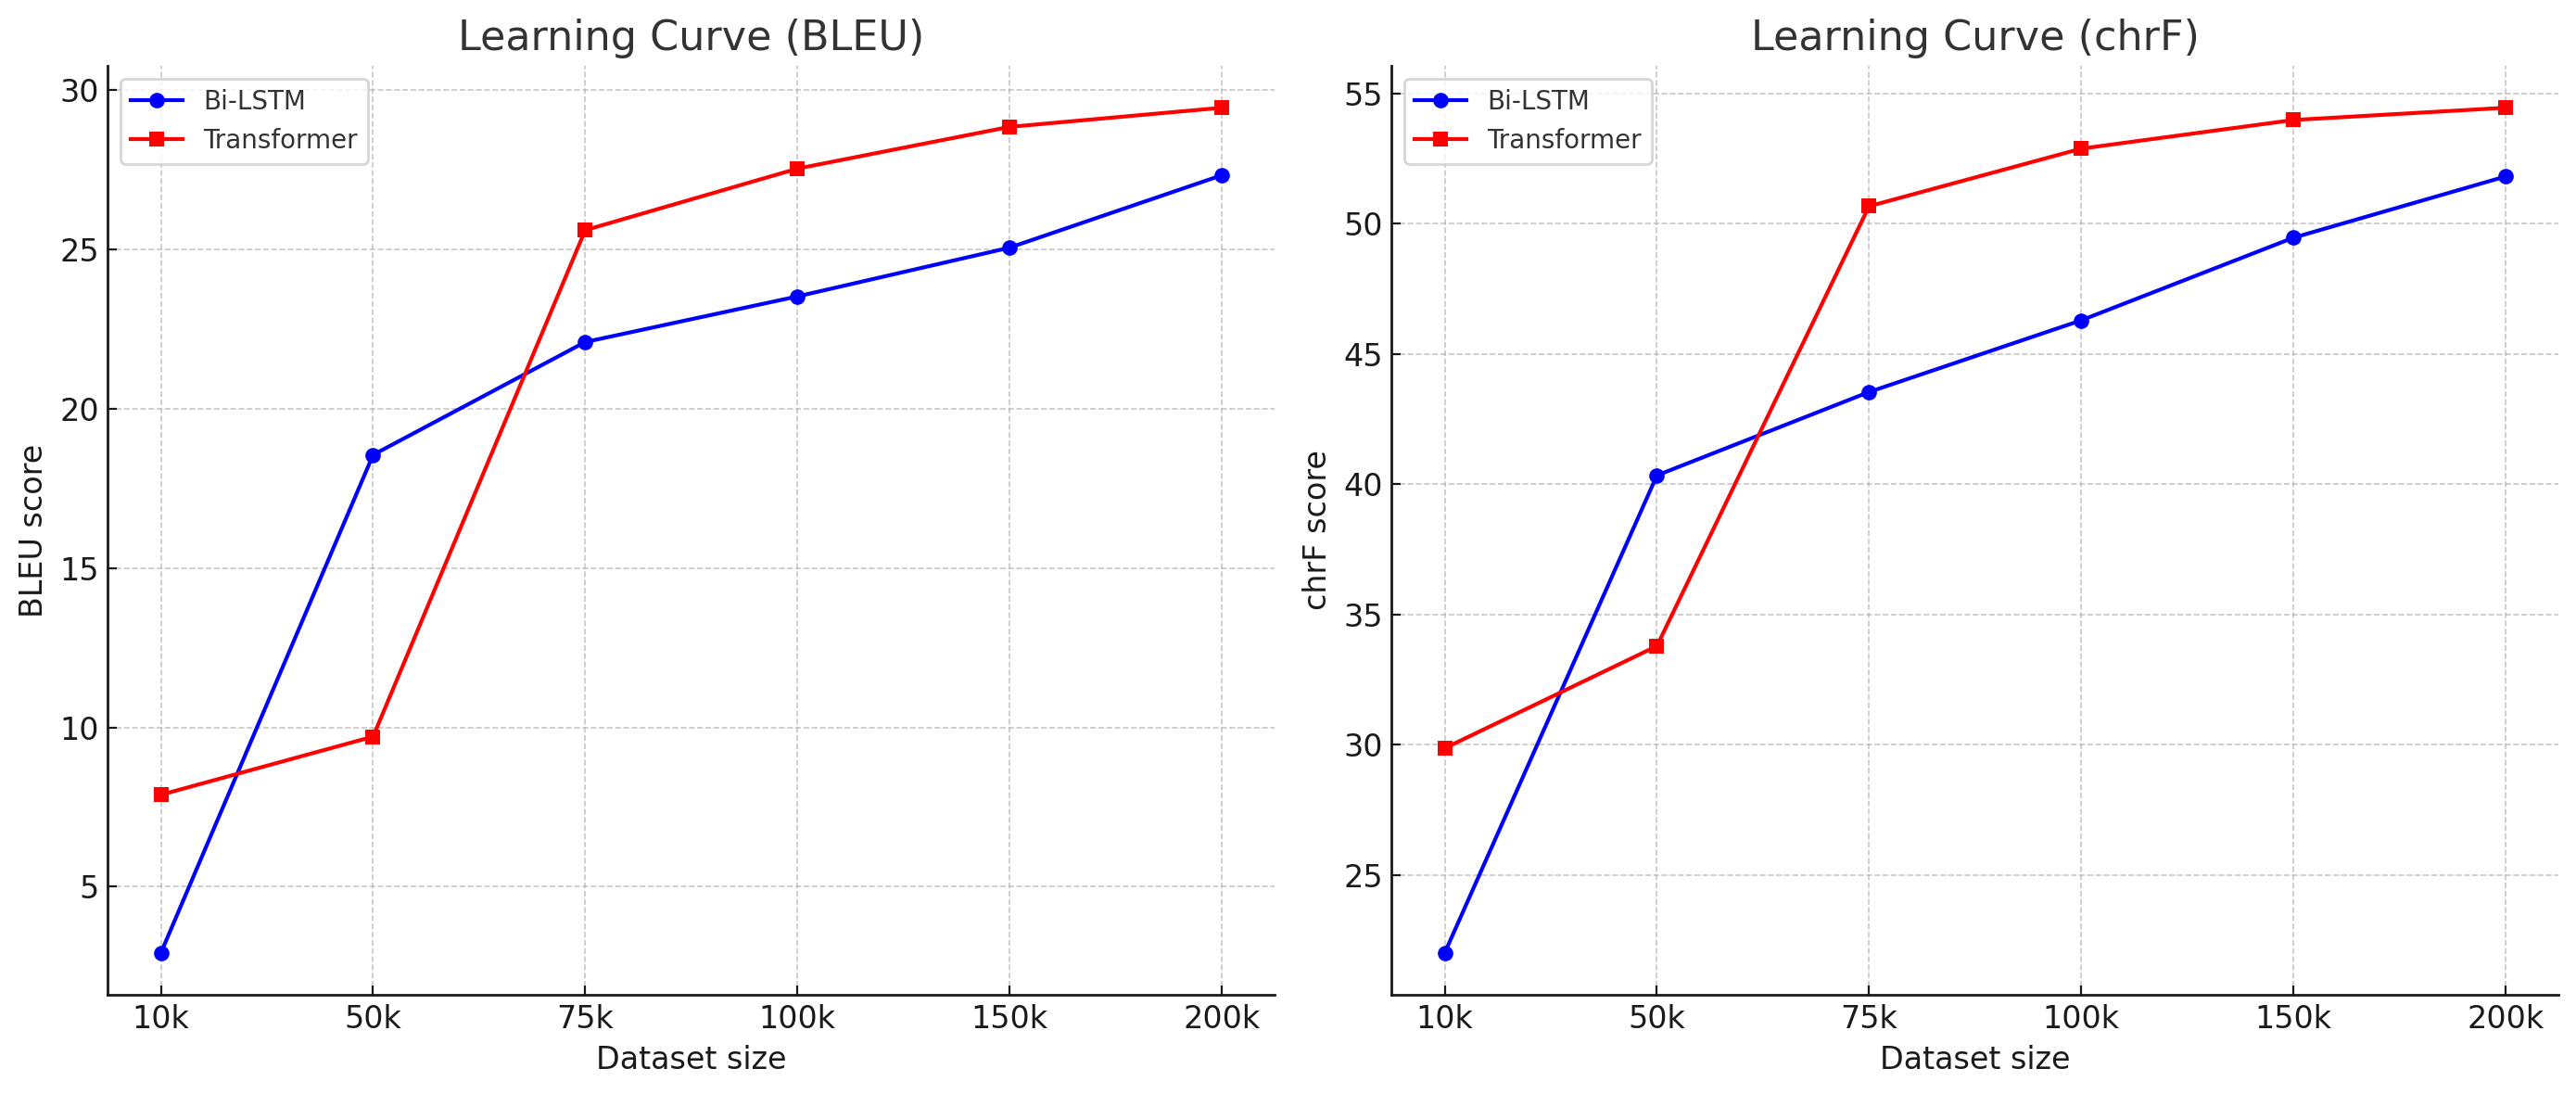
\includegraphics[width=\linewidth]{crossover.png}
\caption{BLEU and chrF scores for Bi-LSTM and Transformer models under varying train dataset sizes}
\label{fig:crossover}
\end{figure}

\section{Conclusion}
\label{sec:conclusion}

We presented a systematic comparison between Bi-LSTM and Transformer models for neural machine translation across varying levels of data availability, simulating low-resource regimes. Through comprehensive hyperparameter tuning and standardized evaluation, we identified a crossover point where Bi-LSTMs outperform Transformers in both BLEU score at 50k sentence pairs and have better computational efficiency between 50k–100k sentence pairs. However, as training data grows beyond 100k, Transformer models achieve higher absolute translation quality, consistent with their known scaling advantages.

These findings suggest that for many truly low-resource languages, where only tens of thousands of parallel sentence pairs exist, Bi-LSTM architectures may be the more effective and compute-efficient choice. Conversely, when moderately sized corpora (e.g., 150k+ pairs) are available, the Transformer regains its edge. Future work should explore whether this crossover trend generalizes across language pairs and domains, and investigate hybrid or adaptive models that can leverage the benefits of both architectures depending on data conditions.


% Bibliography
\bibliographystyle{plain}
\bibliography{references}

\appendix

\section{Appendix}
\subsection{BLEU per GPU-hour}

\begin{table}[H]
\centering
\caption{BLEU per GPU-hour}
\label{table:bleu-gpu-hour}
\begin{tabular}{|l|c|c|c|}
\hline
\textbf{Model} & \textbf{Dataset Size} & \textbf{BLEU} & \textbf{BLEU / GPU-hour} \\
\hline
Bi-LSTM & 10k & 2.93 & 2.93 \\
Bi-LSTM & 50k & 18.55 & 244.27 \\
Bi-LSTM & 75k & 22.09 & 224.72 \\
Bi-LSTM & 100k & 23.52 & 235.20 \\
Bi-LSTM & 150k & 25.05 & 88.91 \\
Bi-LSTM & 200k & 27.32 & 79.95 \\
\hline
Transformer & 10k & 7.89 & 7.89 \\
Transformer & 50k & 9.71 & 14.95 \\
Transformer & 75k & 25.60 & 25.60 \\
Transformer & 100k & 27.53 & 43.47 \\
Transformer & 150k & 28.84 & 48.07 \\
Transformer & 200k & 29.44 & 36.80 \\
\hline
\end{tabular}
\end{table}

\subsection{BLEU per Step}

\begin{table}[H]
\centering
\caption{BLEU per Step}
\label{table:bleu-gpu-step}
\begin{tabular}{|l|c|c|c|}
\hline
\textbf{Model} & \textbf{Dataset Size} & \textbf{BLEU} & \textbf{BLEU / Step} \protect\footnotemark \\
\hline
Bi-LSTM & 10k & 2.93 & 0.0038 \\
Bi-LSTM & 50k & 18.55 & 0.0530 \\
Bi-LSTM & 75k & 22.09 & 0.0497 \\
Bi-LSTM & 100k & 23.52 & 0.0480 \\
Bi-LSTM & 150k & 25.05 & 0.0181 \\
Bi-LSTM & 200k & 27.32 & 0.0156 \\
\hline
Transformer & 10k & 7.89 & 0.0057 \\
Transformer & 50k & 9.71 & 0.0081 \\
Transformer & 75k & 25.60 & 0.0153 \\
Transformer & 100k & 27.53 & 0.0138 \\
Transformer & 150k & 28.84 & 0.0144 \\
Transformer & 200k & 29.44 & 0.0147 \\
\hline
\end{tabular}
\end{table}
\footnotetext{Transformer step counts are halved before computing BLEU/step to account for the different batch sizes used during training.}

\end{document}